\title{Academic career planning using bayesian network}
\author{
        Ray Shulang Lei\\
	200253624\\ 
	Department of Computer Science\\
        University of Regina\\
        Regina, Saskatchewan, S4S0A2, Canada
}
\date{\today}

\documentclass[12pt]{article}
\setlength{\parindent}{0in}
\usepackage{graphicx}
\usepackage{parskip}

\begin{document}
\maketitle

\begin{abstract}
This is the paper's abstract \ldots
\end{abstract}


\section{Introduction}
Using node.js, Dlib C++ Library to build an web application that answers student queries about carrer planning questions.

\section{Design}
Here is a directed acrylic graph A to represent the course prerequisite relations.\\
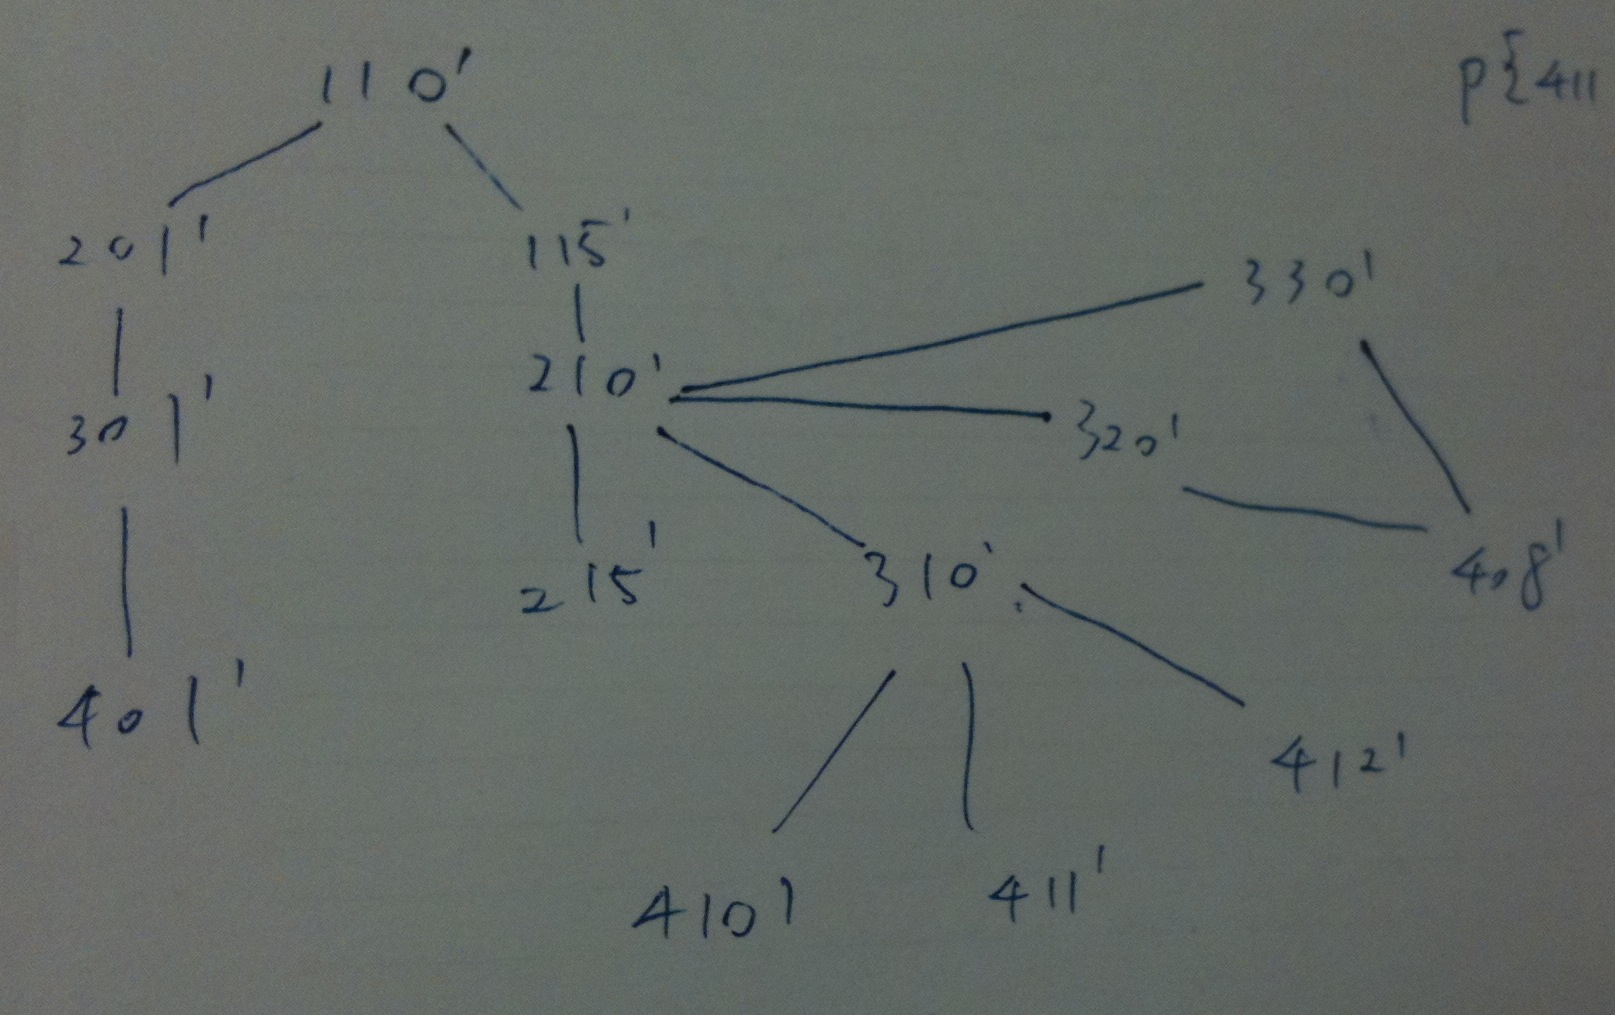
\includegraphics[scale=0.3]{g1_1.jpg}\\

i.e Querying the probability of taking CS411 in the future, provided student have taken CS110:\\
\begin{enumerate}
	\item Search the shortest path between $110'$ to $411'$ in A\\
	\item Which is $110' -> 115' -> 210' -> 310' -> 411'$\\
	\item The length of this path is 4, which means student needs at least 4 semester to finish CS411, provided there is no class not bing offered during these semesters.\\
	\item If there are classes in the path not being offered, we need to add extra semesters accordingly.\\
	\item Run JTP on A, query $P\{CS411 = 1 \mid CS110 = 1\}$\\
	\item Provide feedback to student, telling the least semesters he need to finish CS411 with a probability.\\
\end{enumerate}

\section{Previous work}\label{previous work}
A much longer \LaTeXe{} example was written by Gil~\cite{Gil:02}.

\section{Results}\label{results}
In this section we describe the results.

\section{Conclusions}\label{conclusions}
We worked hard, and achieved very little.

\bibliographystyle{abbrv}
\bibliography{main}
\end{document}

